\section{Robustness Diagnostics and Reproducible Workflow}
\label{app:robustness}

Robustness diagnostics evaluate whether advice-relevant conclusions are stable under
pre-specified alternative structures. This appendix should separate estimation uncertainty
conditional on a reference model from sensitivity across models or scenarios. Generic
scenario comparison, hindcast, ensemble, and projection code should live in packages;
case-study scripts should define scenarios and write results into the content files below.

\subsection{Required R Packages}

\begin{table}

\caption{\label{tab:robustness-libraries}Required R packages for robustness diagnostics.}
\centering
\begin{tabular}[t]{llll}
\toprule
package & role & tier & installed\\
\midrule
knitr & Knit template; format LaTeX tables & core & 1.51\\
r4ss & Read SS3 output across scenarios & run\_code & 1.53.0\\
FLRebuild & curveSS(); scenario time series and process residuals & run\_code & 0.1.0\\
ss3om & readTruth / readFLSss3(); FLR stock objects from SS3 & run\_code & 0.5.3.9004\\
sstruth & retroBacktestData, plotRatios, ssPeDiagnose, plotSpSsb & run\_code & 0.0.0.9020\\
\addlinespace
ggplot2 & Scenario comparison, retrospective, and MVLN figures & run\_code & 4.0.3\\
dplyr & Retrospective trajectory plots (trajMsyLong); MVLN time-series summaries & run\_code & 1.2.1\\
plyr & Summarise scenario outputs (ddply) & run\_code & 1.8.9\\
reshape2 & Reshape scenario tables and MVLN draws (melt/cast) & run\_code & 1.4.5\\
tidyr & Reshape scenario and ensemble tables (planned) & planned & 1.3.2\\
\addlinespace
FLCore & FLR stock objects for status and reference points (planned) & planned & 2.6.29.9001\\
kobe & Kobe-phase plots (planned; ggplot used for MVLN Kobe comparison) & planned & 2.2.0\\
mvtnorm & Multivariate normal sampling for MVLN status uncertainty & run\_code & 1.3.3\\
patchwork & Combine MVLN status time-series panels (optional) & run\_code & 1.3.2\\
\bottomrule
\end{tabular}
\end{table}



\subsection{Scenario Register}

Each robustness appendix should begin with a scenario register. Scenarios should be
pre-specified before reviewing the results, and should identify which uncertainty source
they test.

\begin{table}

\caption{\label{tab:robustness-scenarios}Scenario register for robustness diagnostics (2026 ICCAT shark WG base runs).}
\centering
\begin{tabular}[t]{llllr}
\toprule
scenario & class & purpose & include\_in\_ensemble & weight\\
\midrule
Scenario 1 & reference & Reference assessment (Sc1\_Base) & TRUE & 0.3333333\\
Scenario 2 & structural sensitivity & Alternative structural assumption 1 (Scn02\_base) & TRUE & 0.3333333\\
Scenario 3 & structural sensitivity & Alternative structural assumption 2 (Sc3\_Base) & TRUE & 0.3333333\\
\bottomrule
\end{tabular}
\end{table}


\subsection{Standard Checks}

Robustness reporting should include:

\begin{itemize}
  \item retrospective patterns and hindcast or cross-validation prediction skill;
  \item alternative stock--recruitment, natural mortality, selectivity, catchability, or data-weighting structures;
  \item scenario or ensemble summaries for stock status, reference points, and catch advice;
  \item comparison of model error with estimation error from the reference case;
  \item central tendencies for target reference points and tail probabilities for limit reference points;
  \item rebuilding quantities such as $B_{\mathrm{rebuild}}$, $T_{\mathrm{rebuild}}$, and $P(\mathrm{rebuild\ within\ }T)$ where relevant;
  \item comparison of process-error diagnostics across model classes when ensembles combine biomass-dynamic (JABBA, SPiCT) and age-structured (SS3, SAM) formulations, using a common surplus-production currency on spawning biomass;
  \item hindcast and catch back-test forecast skill where retrospective peels are available.
\end{itemize}

% Robustness diagnostic checks.

\begin{table}

\caption{\label{tab:robustness-pe-summary}Terminal-year scenario status relative to MSY reference points (from curveSS).}
\centering
\begin{tabular}[t]{lrrrr}
\toprule
scenario & terminal\_year & ssb\_bmsy & catch\_msy & harvest\_fmsy\\
\midrule
Scenario 1 & 2023 & 1.07 & 0.429 & 0.401\\
Scenario 2 & 2023 & 1.07 & 0.436 & 0.408\\
Scenario 3 & 2023 & 1.16 & 0.742 & 0.639\\
\bottomrule
\end{tabular}
\end{table}

\begin{table}

\caption{\label{tab:robustness-sspe}Surplus-production misspecification flags by scenario (sstruth::ssPeDiagnose).}
\centering
\begin{tabular}[t]{lrrrrrrrl}
\toprule
scenario & curve\_cor & curve\_rmse & curve\_rel\_rmse & pe\_cor\_ssb & pe\_cor\_biomass & pe\_rmse\_ssb & pe\_rmse\_biomass & likely\_misspecified\\
\midrule
Scenario 1 & 0.9933 & 374.4 & 0.11590 & -0.21360 & 0.2427 & 7.196 & 0.006521 & TRUE\\
Scenario 2 & 0.9816 & 241.1 & 0.07565 & -0.06222 & -0.1129 & 16.800 & 0.007235 & TRUE\\
Scenario 3 & 0.9992 & 1200.0 & 0.64210 & 0.11780 & -0.2070 & 22.950 & 0.007739 & TRUE\\
\bottomrule
\end{tabular}
\end{table}

\begin{table}

\caption{\label{tab:robustness-retro-onestep}One-step-ahead retrospective errors (sstruth::retroBacktestData).}
\centering
\begin{tabular}[t]{llrrlrrrrrrrr}
\toprule
scenario & peel & terminalYr & forecastYr & baseRefEra & catchFore & forecastF & catchEstBaseTime & estFBaseTime & catchReportedData & relErrCatchVsEst & relErrFVsEst & relErrCatchVsReported\\
\midrule
Scenario-2 & 0 & 2023 & 2024 & FORE & 3497 & 0.18070 & 3497 & 0.1807 & 0 & 0.000000 & 0.000000 & NA\\
Scenario-2 & -1 & 2023 & 2024 & FORE & 3246 & 0.18230 & 3497 & 0.1807 & 0 & -0.071670 & 0.008362 & NA\\
Scenario-2 & -2 & 2023 & 2024 & FORE & 0 & 0.00000 & 3497 & 0.1807 & 0 & -1.000000 & -1.000000 & NA\\
Scenario-2 & -3 & 2023 & 2024 & FORE & 3582 & 0.19100 & 3497 & 0.1807 & 0 & 0.024420 & 0.056510 & NA\\
Scenario-2 & -4 & 2023 & 2024 & FORE & 3602 & 0.18690 & 3497 & 0.1807 & 0 & 0.030090 & 0.034030 & NA\\
\addlinespace
Scenario-2 & -5 & 2023 & 2024 & FORE & 3589 & 0.18030 & 3497 & 0.1807 & 0 & 0.026320 & -0.002669 & NA\\
Scenario-2 & -6 & 2023 & 2024 & FORE & 3577 & 0.17500 & 3497 & 0.1807 & 0 & 0.022840 & -0.032010 & NA\\
Scenario-2 & -7 & 2023 & 2024 & FORE & 3557 & 0.17460 & 3497 & 0.1807 & 0 & 0.017130 & -0.033830 & NA\\
Scenario-2 & -8 & 2023 & 2024 & FORE & 3470 & 0.17310 & 3497 & 0.1807 & 0 & -0.007715 & -0.042290 & NA\\
Scenario-2 & -9 & 2023 & 2024 & FORE & 3440 & 0.17280 & 3497 & 0.1807 & 0 & -0.016330 & -0.044060 & NA\\
\addlinespace
Scenario-2 & -10 & 2023 & 2024 & FORE & 3455 & 0.17330 & 3497 & 0.1807 & 0 & -0.011900 & -0.041230 & NA\\
Scenario-3 & 0 & 2023 & 2024 & FORE & 2056 & 0.08000 & 2056 & 0.0800 & 0 & 0.000000 & 0.000000 & NA\\
Scenario-3 & -1 & 2023 & 2024 & FORE & 0 & 0.00000 & 2056 & 0.0800 & 0 & -1.000000 & -1.000000 & NA\\
Scenario-3 & -2 & 2023 & 2024 & FORE & 1896 & 0.08577 & 2056 & 0.0800 & 0 & -0.077730 & 0.072210 & NA\\
Scenario-3 & -3 & 2023 & 2024 & FORE & 2032 & 0.08570 & 2056 & 0.0800 & 0 & -0.011440 & 0.071250 & NA\\
\addlinespace
Scenario-3 & -4 & 2023 & 2024 & FORE & 1927 & 0.08428 & 2056 & 0.0800 & 0 & -0.062570 & 0.053610 & NA\\
Scenario-3 & -5 & 2023 & 2024 & FORE & 1856 & 0.08289 & 2056 & 0.0800 & 0 & -0.097490 & 0.036150 & NA\\
Scenario-3 & -6 & 2023 & 2024 & FORE & 1780 & 0.08138 & 2056 & 0.0800 & 0 & -0.134400 & 0.017320 & NA\\
Scenario-3 & -7 & 2023 & 2024 & FORE & 1806 & 0.08284 & 2056 & 0.0800 & 0 & -0.121600 & 0.035590 & NA\\
Scenario-3 & -8 & 2023 & 2024 & FORE & 1722 & 0.08392 & 2056 & 0.0800 & 0 & -0.162600 & 0.049080 & NA\\
\addlinespace
Scenario-3 & -9 & 2023 & 2024 & FORE & 1542 & 0.08266 & 2056 & 0.0800 & 0 & -0.250200 & 0.033260 & NA\\
Scenario-3 & -10 & 2023 & 2024 & FORE & 1507 & 0.08584 & 2056 & 0.0800 & 0 & -0.267200 & 0.073090 & NA\\
\bottomrule
\end{tabular}
\end{table}

\begin{table}

\caption{\label{tab:robustness-mvln-terminal}Terminal-year MVLN status uncertainty by scenario (year 2023). Harvest = F/FMSY from Hessian draws.}
\centering
\begin{tabular}[t]{llrrrrrrrrrr}
\toprule
  & scenario & terminal\_year & stock\_median & stock\_p05 & stock\_p95 & harvest\_median & harvest\_p05 & harvest\_p95 & p\_overfished & p\_overfishing & weight\\
\midrule
Scenario-1 & Scenario-1 & 2023 & 1.05 & 0.867 & 1.32 & 24.3 & 21.0 & 27.9 & 0.326 & 1 & 0.333\\
Scenario-2 & Scenario-2 & 2023 & 1.06 & 0.926 & 1.22 & 25.4 & 23.1 & 28.1 & 0.220 & 1 & 0.333\\
Scenario-3 & Scenario-3 & 2023 & 1.16 & 0.938 & 1.42 & 43.3 & 35.5 & 52.7 & 0.112 & 1 & 0.333\\
\bottomrule
\end{tabular}
\end{table}

\begin{table}

\caption{\label{tab:robustness-catch-backtest}Catch back-test forecast summaries by peel and forecast scenario (collected via run-catch-backtests.R).}
\centering
\begin{tabular}[t]{lllrrrrll}
\toprule
scenario & peel & forecast\_scenario & forecast\_year & spawn\_bio & dead\_catch & sum\_f & run\_dir & ok\\
\midrule
Scenario-2 & 0 & catchReported & 2024 & 1188.0 & NA & NA & C:/active/flr/sstruth/data/ss3/sma-natl/Scenario-2/retrospectives/retro0/catchReported & TRUE\\
Scenario-2 & 0 & fMeanFull & 2024 & 1188.0 & NA & NA & C:/active/flr/sstruth/data/ss3/sma-natl/Scenario-2/retrospectives/retro0/fMeanFull & TRUE\\
Scenario-2 & 0 & fZero & 2024 & 1188.0 & NA & NA & C:/active/flr/sstruth/data/ss3/sma-natl/Scenario-2/retrospectives/retro0/fZero & TRUE\\
Scenario-2 & 0 & fMsy & 2024 & 1188.0 & NA & NA & C:/active/flr/sstruth/data/ss3/sma-natl/Scenario-2/retrospectives/retro0/fMsy & TRUE\\
Scenario-2 & -1 & catchReported & 2024 & 1184.0 & NA & NA & C:/active/flr/sstruth/data/ss3/sma-natl/Scenario-2/retrospectives/retro-1/catchReported & TRUE\\
\addlinespace
Scenario-2 & -1 & fMeanFull & 2024 & 1184.0 & NA & NA & C:/active/flr/sstruth/data/ss3/sma-natl/Scenario-2/retrospectives/retro-1/fMeanFull & TRUE\\
Scenario-2 & -1 & fZero & 2024 & 1184.0 & NA & NA & C:/active/flr/sstruth/data/ss3/sma-natl/Scenario-2/retrospectives/retro-1/fZero & TRUE\\
Scenario-2 & -1 & fMsy & 2024 & 1184.0 & NA & NA & C:/active/flr/sstruth/data/ss3/sma-natl/Scenario-2/retrospectives/retro-1/fMsy & TRUE\\
Scenario-2 & -2 & catchReported & 2024 & 1243.0 & NA & NA & C:/active/flr/sstruth/data/ss3/sma-natl/Scenario-2/retrospectives/retro-2/catchReported & TRUE\\
Scenario-2 & -2 & fMeanFull & 2024 & 1243.0 & NA & NA & C:/active/flr/sstruth/data/ss3/sma-natl/Scenario-2/retrospectives/retro-2/fMeanFull & TRUE\\
\addlinespace
Scenario-2 & -2 & fZero & 2024 & 1243.0 & NA & NA & C:/active/flr/sstruth/data/ss3/sma-natl/Scenario-2/retrospectives/retro-2/fZero & TRUE\\
Scenario-2 & -2 & fMsy & 2024 & 1243.0 & NA & NA & C:/active/flr/sstruth/data/ss3/sma-natl/Scenario-2/retrospectives/retro-2/fMsy & TRUE\\
Scenario-2 & -3 & catchReported & 2024 & 1252.0 & NA & NA & C:/active/flr/sstruth/data/ss3/sma-natl/Scenario-2/retrospectives/retro-3/catchReported & TRUE\\
Scenario-2 & -3 & fMeanFull & 2024 & 1252.0 & NA & NA & C:/active/flr/sstruth/data/ss3/sma-natl/Scenario-2/retrospectives/retro-3/fMeanFull & TRUE\\
Scenario-2 & -3 & fZero & 2024 & 1252.0 & NA & NA & C:/active/flr/sstruth/data/ss3/sma-natl/Scenario-2/retrospectives/retro-3/fZero & TRUE\\
\addlinespace
Scenario-2 & -3 & fMsy & 2024 & 1252.0 & NA & NA & C:/active/flr/sstruth/data/ss3/sma-natl/Scenario-2/retrospectives/retro-3/fMsy & TRUE\\
Scenario-2 & -4 & catchReported & 2024 & 1238.0 & NA & NA & C:/active/flr/sstruth/data/ss3/sma-natl/Scenario-2/retrospectives/retro-4/catchReported & TRUE\\
Scenario-2 & -4 & fMeanFull & 2024 & 1238.0 & NA & NA & C:/active/flr/sstruth/data/ss3/sma-natl/Scenario-2/retrospectives/retro-4/fMeanFull & TRUE\\
Scenario-2 & -4 & fZero & 2024 & 1238.0 & NA & NA & C:/active/flr/sstruth/data/ss3/sma-natl/Scenario-2/retrospectives/retro-4/fZero & TRUE\\
Scenario-2 & -4 & fMsy & 2024 & 1238.0 & NA & NA & C:/active/flr/sstruth/data/ss3/sma-natl/Scenario-2/retrospectives/retro-4/fMsy & TRUE\\
\addlinespace
Scenario-2 & -5 & catchReported & 2024 & 1203.0 & NA & NA & C:/active/flr/sstruth/data/ss3/sma-natl/Scenario-2/retrospectives/retro-5/catchReported & TRUE\\
Scenario-2 & -5 & fMeanFull & 2024 & 1203.0 & NA & NA & C:/active/flr/sstruth/data/ss3/sma-natl/Scenario-2/retrospectives/retro-5/fMeanFull & TRUE\\
Scenario-2 & -5 & fZero & 2024 & 1203.0 & NA & NA & C:/active/flr/sstruth/data/ss3/sma-natl/Scenario-2/retrospectives/retro-5/fZero & TRUE\\
Scenario-2 & -5 & fMsy & 2024 & 1203.0 & NA & NA & C:/active/flr/sstruth/data/ss3/sma-natl/Scenario-2/retrospectives/retro-5/fMsy & TRUE\\
Scenario-2 & -6 & catchReported & 2024 & 1196.0 & NA & NA & C:/active/flr/sstruth/data/ss3/sma-natl/Scenario-2/retrospectives/retro-6/catchReported & TRUE\\
\addlinespace
Scenario-2 & -6 & fMeanFull & 2024 & 1196.0 & NA & NA & C:/active/flr/sstruth/data/ss3/sma-natl/Scenario-2/retrospectives/retro-6/fMeanFull & TRUE\\
Scenario-2 & -6 & fZero & 2024 & 1196.0 & NA & NA & C:/active/flr/sstruth/data/ss3/sma-natl/Scenario-2/retrospectives/retro-6/fZero & TRUE\\
Scenario-2 & -6 & fMsy & 2024 & 1196.0 & NA & NA & C:/active/flr/sstruth/data/ss3/sma-natl/Scenario-2/retrospectives/retro-6/fMsy & TRUE\\
Scenario-2 & -7 & catchReported & 2024 & 1160.0 & NA & NA & C:/active/flr/sstruth/data/ss3/sma-natl/Scenario-2/retrospectives/retro-7/catchReported & TRUE\\
Scenario-2 & -7 & fMeanFull & 2024 & 1160.0 & NA & NA & C:/active/flr/sstruth/data/ss3/sma-natl/Scenario-2/retrospectives/retro-7/fMeanFull & TRUE\\
\addlinespace
Scenario-2 & -7 & fZero & 2024 & 1160.0 & NA & NA & C:/active/flr/sstruth/data/ss3/sma-natl/Scenario-2/retrospectives/retro-7/fZero & TRUE\\
Scenario-2 & -7 & fMsy & 2024 & 1160.0 & NA & NA & C:/active/flr/sstruth/data/ss3/sma-natl/Scenario-2/retrospectives/retro-7/fMsy & TRUE\\
Scenario-2 & -8 & catchReported & 2024 & 1116.0 & NA & NA & C:/active/flr/sstruth/data/ss3/sma-natl/Scenario-2/retrospectives/retro-8/catchReported & TRUE\\
Scenario-2 & -8 & fMeanFull & 2024 & 1116.0 & NA & NA & C:/active/flr/sstruth/data/ss3/sma-natl/Scenario-2/retrospectives/retro-8/fMeanFull & TRUE\\
Scenario-2 & -8 & fZero & 2024 & 1116.0 & NA & NA & C:/active/flr/sstruth/data/ss3/sma-natl/Scenario-2/retrospectives/retro-8/fZero & TRUE\\
\addlinespace
Scenario-2 & -8 & fMsy & 2024 & 1116.0 & NA & NA & C:/active/flr/sstruth/data/ss3/sma-natl/Scenario-2/retrospectives/retro-8/fMsy & TRUE\\
Scenario-2 & -9 & catchReported & 2024 & 1089.0 & NA & NA & C:/active/flr/sstruth/data/ss3/sma-natl/Scenario-2/retrospectives/retro-9/catchReported & TRUE\\
Scenario-2 & -9 & fMeanFull & 2024 & 1089.0 & NA & NA & C:/active/flr/sstruth/data/ss3/sma-natl/Scenario-2/retrospectives/retro-9/fMeanFull & TRUE\\
Scenario-2 & -9 & fZero & 2024 & 1089.0 & NA & NA & C:/active/flr/sstruth/data/ss3/sma-natl/Scenario-2/retrospectives/retro-9/fZero & TRUE\\
Scenario-2 & -9 & fMsy & 2024 & 1089.0 & NA & NA & C:/active/flr/sstruth/data/ss3/sma-natl/Scenario-2/retrospectives/retro-9/fMsy & TRUE\\
\addlinespace
Scenario-2 & -10 & catchReported & 2024 & 1079.0 & NA & NA & C:/active/flr/sstruth/data/ss3/sma-natl/Scenario-2/retrospectives/retro-10/catchReported & TRUE\\
Scenario-2 & -10 & fMeanFull & 2024 & 1079.0 & NA & NA & C:/active/flr/sstruth/data/ss3/sma-natl/Scenario-2/retrospectives/retro-10/fMeanFull & TRUE\\
Scenario-2 & -10 & fZero & 2024 & 1079.0 & NA & NA & C:/active/flr/sstruth/data/ss3/sma-natl/Scenario-2/retrospectives/retro-10/fZero & TRUE\\
Scenario-2 & -10 & fMsy & 2024 & 1079.0 & NA & NA & C:/active/flr/sstruth/data/ss3/sma-natl/Scenario-2/retrospectives/retro-10/fMsy & TRUE\\
Scenario-3 & 0 & catchReported & 2024 & 451.1 & NA & NA & C:/active/flr/sstruth/data/ss3/sma-natl/Scenario-3/retrospectives/retro0/catchReported & TRUE\\
\addlinespace
Scenario-3 & 0 & fMeanFull & 2024 & 451.1 & NA & NA & C:/active/flr/sstruth/data/ss3/sma-natl/Scenario-3/retrospectives/retro0/fMeanFull & TRUE\\
Scenario-3 & 0 & fZero & 2024 & 451.1 & NA & NA & C:/active/flr/sstruth/data/ss3/sma-natl/Scenario-3/retrospectives/retro0/fZero & TRUE\\
Scenario-3 & 0 & fMsy & 2024 & 451.1 & NA & NA & C:/active/flr/sstruth/data/ss3/sma-natl/Scenario-3/retrospectives/retro0/fMsy & TRUE\\
Scenario-3 & -1 & catchReported & 2024 & 447.3 & NA & NA & C:/active/flr/sstruth/data/ss3/sma-natl/Scenario-3/retrospectives/retro-1/catchReported & TRUE\\
Scenario-3 & -1 & fMeanFull & 2024 & 447.3 & NA & NA & C:/active/flr/sstruth/data/ss3/sma-natl/Scenario-3/retrospectives/retro-1/fMeanFull & TRUE\\
\addlinespace
Scenario-3 & -1 & fZero & 2024 & 447.3 & NA & NA & C:/active/flr/sstruth/data/ss3/sma-natl/Scenario-3/retrospectives/retro-1/fZero & TRUE\\
Scenario-3 & -1 & fMsy & 2024 & 447.3 & NA & NA & C:/active/flr/sstruth/data/ss3/sma-natl/Scenario-3/retrospectives/retro-1/fMsy & TRUE\\
Scenario-3 & -2 & catchReported & 2024 & 472.4 & NA & NA & C:/active/flr/sstruth/data/ss3/sma-natl/Scenario-3/retrospectives/retro-2/catchReported & TRUE\\
Scenario-3 & -2 & fMeanFull & 2024 & 472.4 & NA & NA & C:/active/flr/sstruth/data/ss3/sma-natl/Scenario-3/retrospectives/retro-2/fMeanFull & TRUE\\
Scenario-3 & -2 & fZero & 2024 & 472.4 & NA & NA & C:/active/flr/sstruth/data/ss3/sma-natl/Scenario-3/retrospectives/retro-2/fZero & TRUE\\
\addlinespace
Scenario-3 & -2 & fMsy & 2024 & 472.4 & NA & NA & C:/active/flr/sstruth/data/ss3/sma-natl/Scenario-3/retrospectives/retro-2/fMsy & TRUE\\
Scenario-3 & -3 & catchReported & 2024 & 471.4 & NA & NA & C:/active/flr/sstruth/data/ss3/sma-natl/Scenario-3/retrospectives/retro-3/catchReported & TRUE\\
Scenario-3 & -3 & fMeanFull & 2024 & 471.4 & NA & NA & C:/active/flr/sstruth/data/ss3/sma-natl/Scenario-3/retrospectives/retro-3/fMeanFull & TRUE\\
Scenario-3 & -3 & fZero & 2024 & 471.4 & NA & NA & C:/active/flr/sstruth/data/ss3/sma-natl/Scenario-3/retrospectives/retro-3/fZero & TRUE\\
Scenario-3 & -3 & fMsy & 2024 & 471.4 & NA & NA & C:/active/flr/sstruth/data/ss3/sma-natl/Scenario-3/retrospectives/retro-3/fMsy & TRUE\\
\addlinespace
Scenario-3 & -4 & catchReported & 2024 & 463.6 & NA & NA & C:/active/flr/sstruth/data/ss3/sma-natl/Scenario-3/retrospectives/retro-4/catchReported & TRUE\\
Scenario-3 & -4 & fMeanFull & 2024 & 463.6 & NA & NA & C:/active/flr/sstruth/data/ss3/sma-natl/Scenario-3/retrospectives/retro-4/fMeanFull & TRUE\\
Scenario-3 & -4 & fZero & 2024 & 463.6 & NA & NA & C:/active/flr/sstruth/data/ss3/sma-natl/Scenario-3/retrospectives/retro-4/fZero & TRUE\\
Scenario-3 & -4 & fMsy & 2024 & 463.6 & NA & NA & C:/active/flr/sstruth/data/ss3/sma-natl/Scenario-3/retrospectives/retro-4/fMsy & TRUE\\
Scenario-3 & -5 & catchReported & 2024 & 448.2 & NA & NA & C:/active/flr/sstruth/data/ss3/sma-natl/Scenario-3/retrospectives/retro-5/catchReported & TRUE\\
\addlinespace
Scenario-3 & -5 & fMeanFull & 2024 & 448.2 & NA & NA & C:/active/flr/sstruth/data/ss3/sma-natl/Scenario-3/retrospectives/retro-5/fMeanFull & TRUE\\
Scenario-3 & -5 & fZero & 2024 & 448.2 & NA & NA & C:/active/flr/sstruth/data/ss3/sma-natl/Scenario-3/retrospectives/retro-5/fZero & TRUE\\
Scenario-3 & -5 & fMsy & 2024 & 448.2 & NA & NA & C:/active/flr/sstruth/data/ss3/sma-natl/Scenario-3/retrospectives/retro-5/fMsy & TRUE\\
Scenario-3 & -6 & catchReported & 2024 & 436.5 & NA & NA & C:/active/flr/sstruth/data/ss3/sma-natl/Scenario-3/retrospectives/retro-6/catchReported & TRUE\\
Scenario-3 & -6 & fMeanFull & 2024 & 436.5 & NA & NA & C:/active/flr/sstruth/data/ss3/sma-natl/Scenario-3/retrospectives/retro-6/fMeanFull & TRUE\\
\addlinespace
Scenario-3 & -6 & fZero & 2024 & 436.5 & NA & NA & C:/active/flr/sstruth/data/ss3/sma-natl/Scenario-3/retrospectives/retro-6/fZero & TRUE\\
Scenario-3 & -6 & fMsy & 2024 & 436.5 & NA & NA & C:/active/flr/sstruth/data/ss3/sma-natl/Scenario-3/retrospectives/retro-6/fMsy & TRUE\\
Scenario-3 & -7 & catchReported & 2024 & 435.6 & NA & NA & C:/active/flr/sstruth/data/ss3/sma-natl/Scenario-3/retrospectives/retro-7/catchReported & TRUE\\
Scenario-3 & -7 & fMeanFull & 2024 & 435.6 & NA & NA & C:/active/flr/sstruth/data/ss3/sma-natl/Scenario-3/retrospectives/retro-7/fMeanFull & TRUE\\
Scenario-3 & -7 & fZero & 2024 & 435.6 & NA & NA & C:/active/flr/sstruth/data/ss3/sma-natl/Scenario-3/retrospectives/retro-7/fZero & TRUE\\
\addlinespace
Scenario-3 & -7 & fMsy & 2024 & 435.6 & NA & NA & C:/active/flr/sstruth/data/ss3/sma-natl/Scenario-3/retrospectives/retro-7/fMsy & TRUE\\
Scenario-3 & -8 & catchReported & 2024 & 415.5 & NA & NA & C:/active/flr/sstruth/data/ss3/sma-natl/Scenario-3/retrospectives/retro-8/catchReported & TRUE\\
Scenario-3 & -8 & fMeanFull & 2024 & 415.5 & NA & NA & C:/active/flr/sstruth/data/ss3/sma-natl/Scenario-3/retrospectives/retro-8/fMeanFull & TRUE\\
Scenario-3 & -8 & fZero & 2024 & 415.5 & NA & NA & C:/active/flr/sstruth/data/ss3/sma-natl/Scenario-3/retrospectives/retro-8/fZero & TRUE\\
Scenario-3 & -8 & fMsy & 2024 & 415.5 & NA & NA & C:/active/flr/sstruth/data/ss3/sma-natl/Scenario-3/retrospectives/retro-8/fMsy & TRUE\\
\addlinespace
Scenario-3 & -9 & catchReported & 2024 & 380.5 & NA & NA & C:/active/flr/sstruth/data/ss3/sma-natl/Scenario-3/retrospectives/retro-9/catchReported & TRUE\\
Scenario-3 & -9 & fMeanFull & 2024 & 380.5 & NA & NA & C:/active/flr/sstruth/data/ss3/sma-natl/Scenario-3/retrospectives/retro-9/fMeanFull & TRUE\\
Scenario-3 & -9 & fZero & 2024 & 380.5 & NA & NA & C:/active/flr/sstruth/data/ss3/sma-natl/Scenario-3/retrospectives/retro-9/fZero & TRUE\\
Scenario-3 & -9 & fMsy & 2024 & 380.5 & NA & NA & C:/active/flr/sstruth/data/ss3/sma-natl/Scenario-3/retrospectives/retro-9/fMsy & TRUE\\
Scenario-3 & -10 & catchReported & 2024 & 356.2 & NA & NA & C:/active/flr/sstruth/data/ss3/sma-natl/Scenario-3/retrospectives/retro-10/catchReported & TRUE\\
\addlinespace
Scenario-3 & -10 & fMeanFull & 2024 & 356.2 & NA & NA & C:/active/flr/sstruth/data/ss3/sma-natl/Scenario-3/retrospectives/retro-10/fMeanFull & TRUE\\
Scenario-3 & -10 & fZero & 2024 & 356.2 & NA & NA & C:/active/flr/sstruth/data/ss3/sma-natl/Scenario-3/retrospectives/retro-10/fZero & TRUE\\
Scenario-3 & -10 & fMsy & 2024 & 356.2 & NA & NA & C:/active/flr/sstruth/data/ss3/sma-natl/Scenario-3/retrospectives/retro-10/fMsy & TRUE\\
\bottomrule
\end{tabular}
\end{table}



\subsection{Diagnostic Output}

Tables, figures, and code-generated summaries can be added to the file below as they
become available.

% Robustness diagnostic figures.

\begin{figure}[H]
  \centering
  \includegraphics[width=0.92\linewidth]{appendices/figs/robustness/ss3-ts.png}
  \caption{SS3 scenario time series relative to MSY reference points.}
  \label{fig:robustness-ss3-ts}
\end{figure}

\begin{figure}[H]
  \centering
  \includegraphics[width=0.92\linewidth]{appendices/figs/robustness/ss3-res-time.png}
  \caption{Process residuals by scenario (from curveSS).}
  \label{fig:robustness-ss3-res-time}
\end{figure}

\begin{figure}[H]
  \centering
  \includegraphics[width=0.92\linewidth]{appendices/figs/robustness/ss3-res-acf.png}
  \caption{ACF of process residuals by scenario.}
  \label{fig:robustness-ss3-res-acf}
\end{figure}

\begin{figure}[H]
  \centering
  \includegraphics[width=0.95\linewidth]{appendices/figs/robustness/retro-traj-msy.png}
  \caption{Retrospective peel trajectories vs MSY benchmarks (sstruth::retroBacktestData).}
  \label{fig:robustness-retro-traj}
\end{figure}

\begin{figure}[H]
  \centering
  \includegraphics[width=0.92\linewidth]{appendices/figs/robustness/retro-bratio-horizon.png}
  \caption{Multi-horizon SSB/BMSY retrospective ratios (sstruth::plotRatios).}
  \label{fig:robustness-retro-bratio}
\end{figure}

\begin{figure}[H]
  \centering
  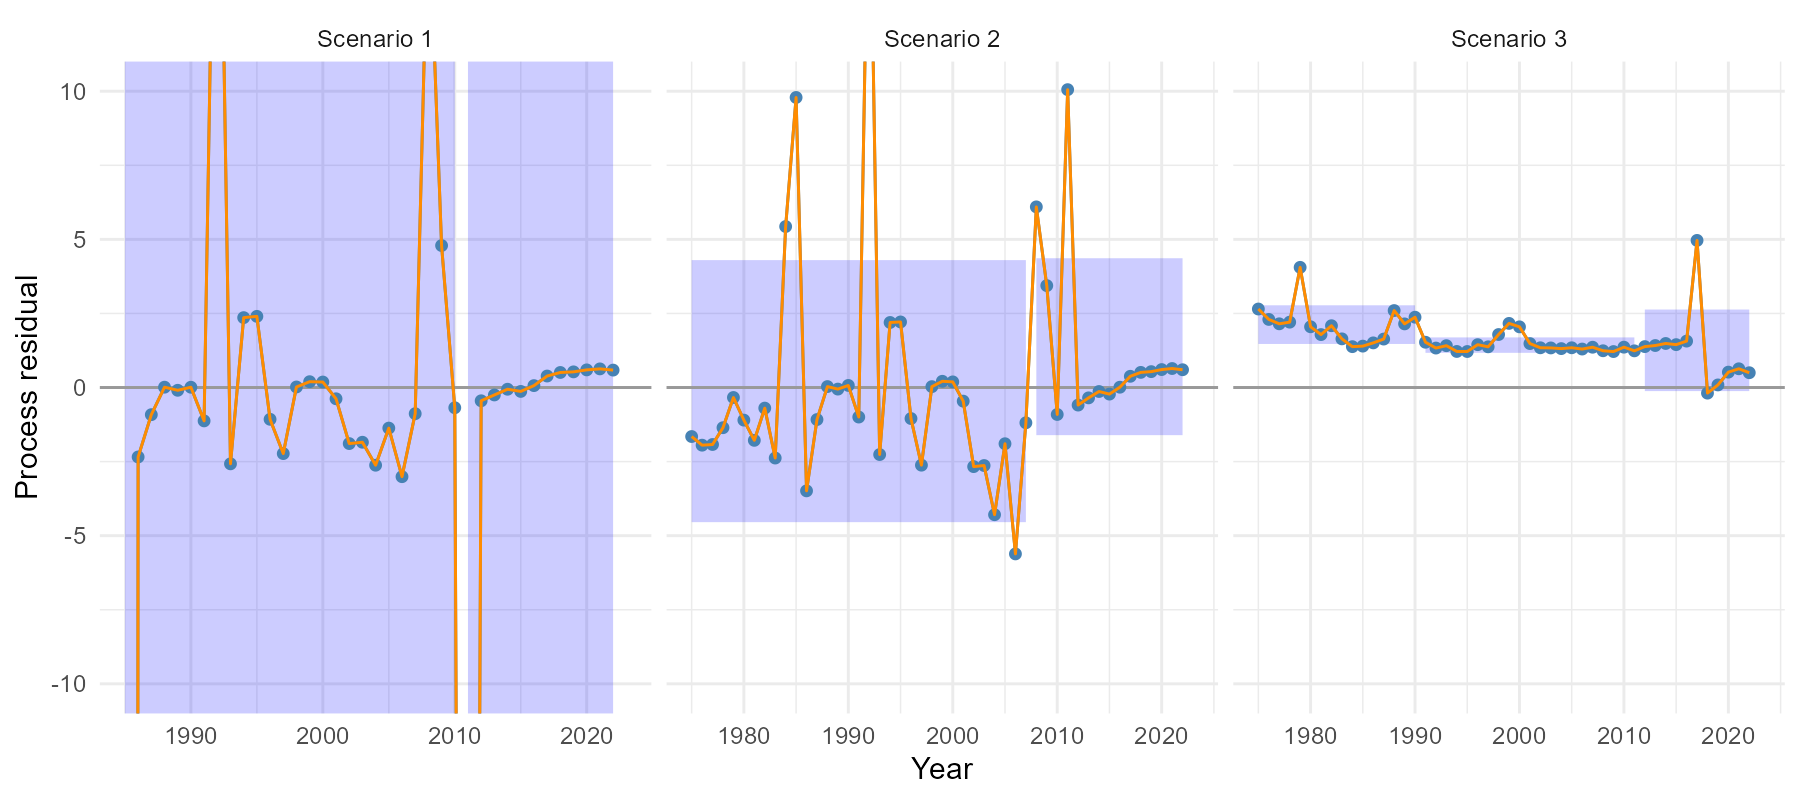
\includegraphics[width=0.92\linewidth]{figs/sma-fig-res-time-1.png}
  \caption{sma fig res time 1}
  \label{fig:robustness-sma-fig-res-time-1}
\end{figure}

\begin{figure}[H]
  \centering
  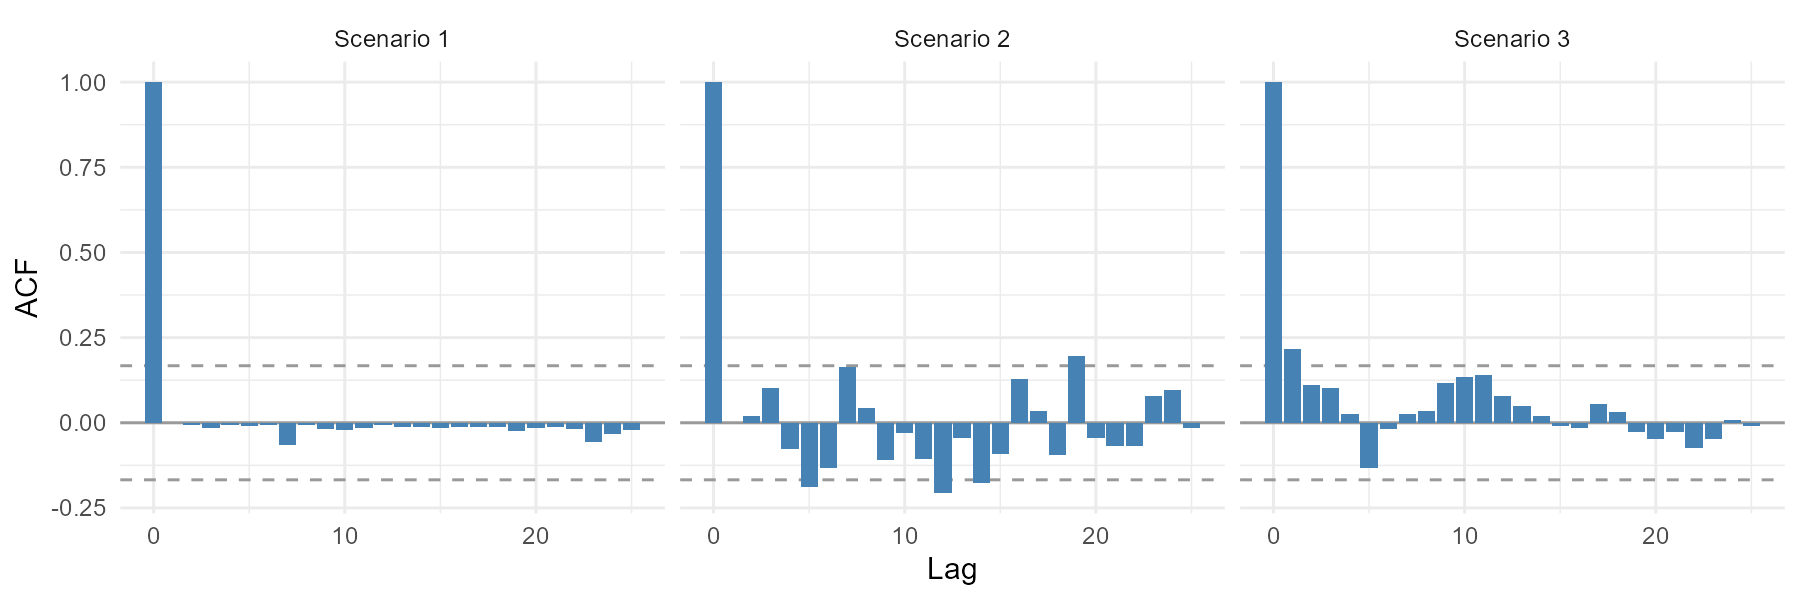
\includegraphics[width=0.92\linewidth]{figs/sma-fig-res-acf-1.png}
  \caption{sma fig res acf 1}
  \label{fig:robustness-sma-fig-res-acf-1}
\end{figure}



\subsection{Best Assessment Versus Ensemble}

If the estimates from pre-specified alternative models remain within the uncertainty
intervals of the reference model for the management quantities of interest, a best
assessment may be adequate for advice. If model sensitivity is larger than estimation
uncertainty, especially for limit tail probabilities or target central tendencies, advice is
model-dependent and should be reported using a scenario set or ensemble.

% Best-assessment versus ensemble comparison (MVLN).

% Reference scenario: Scenario-1; MVLN Monte Carlo draws = 500 per scenario.

\begin{table}

\caption{\label{tab:robustness-mvln-ensemble}MVLN terminal status and tail probabilities (year 2023). Compare estimation uncertainty (reference) with structural sensitivity scenarios.}
\centering
\begin{tabular}[t]{llrrrrrrrrrr}
\toprule
  & scenario & terminal\_year & stock\_median & stock\_p05 & stock\_p95 & harvest\_median & harvest\_p05 & harvest\_p95 & p\_overfished & p\_overfishing & weight\\
\midrule
Scenario-1 & Scenario-1 & 2023 & 1.05 & 0.867 & 1.32 & 24.3 & 21.0 & 27.9 & 0.326 & 1 & 0.333\\
Scenario-2 & Scenario-2 & 2023 & 1.06 & 0.926 & 1.22 & 25.4 & 23.1 & 28.1 & 0.220 & 1 & 0.333\\
Scenario-3 & Scenario-3 & 2023 & 1.16 & 0.938 & 1.42 & 43.3 & 35.5 & 52.7 & 0.112 & 1 & 0.333\\
\bottomrule
\end{tabular}
\end{table}

\begin{table}

\caption{\label{tab:robustness-ensemble-weight-comparison}Ensemble weight comparison by scenario: (i) equal weights; (ii) ICES-style Akaike weights $w_i \propto \exp(-\Delta\mathrm{AIC}/2)$ from total SS3 negative log-likelihood (comparable models); (iii) CVindexmase; (iv) CVindexrho (hindcast skill from retrospective peels; Scenarios 2--3 only until LOO CPUE is collected).}
\centering
\begin{tabular}[t]{lrrrr}
\toprule
scenario & w\_equal & w\_ices & w\_cvindexmase & w\_cvindexrho\\
\midrule
Scenario-1 & 0.3333 & 0 & NA & NA\\
Scenario-2 & 0.3333 & 1 & 1 & 0.6667\\
Scenario-3 & 0.3333 & 0 & 0 & 0.3333\\
\bottomrule
\end{tabular}
\end{table}

\begin{figure}[H]
  \centering
  \includegraphics[width=0.92\linewidth]{appendices/figs/robustness/mvln-kobe-terminal.png}
  \caption{Terminal-year Kobe-style comparison of MVLN draws: reference (Scenario-1) vs structural sensitivity scenarios.}
  \label{fig:robustness-mvln-kobe}
\end{figure}

\begin{figure}[H]
  \centering
  \includegraphics[width=0.92\linewidth]{appendices/figs/robustness/mvln-terminal-compare.png}
  \caption{Terminal MVLN medians and 5--95\% intervals for SSB/BMSY and F/FMSY by scenario.}
  \label{fig:robustness-mvln-terminal}
\end{figure}

\begin{figure}[H]
  \centering
  \includegraphics[width=0.92\linewidth]{appendices/figs/robustness/mvln-status-ts.png}
  \caption{Recent-year MVLN status trajectories with 5--95\% intervals by scenario.}
  \label{fig:robustness-mvln-ts}
\end{figure}



\subsection{Interpretation}

State which advice quantities are robust, which are model-dependent, and whether the
case study should be presented as a best assessment, a screened scenario set, an ensemble,
or an MSE operating-model set.

% Case-specific robustness interpretation.
% State which advice quantities are robust, which are model-dependent,
% and whether reporting should use a best assessment, screened scenario set, or ensemble.


